\documentclass{report}
\usepackage[margin=1in, paperwidth=8.5in, paperheight=11in]{geometry}
%Math packages%
\usepackage{amsmath}
\usepackage{amsthm}
%Spacing%
\usepackage{setspace}
\onehalfspacing
%Lecture number%
\newcommand{\lectureNum}{7}
%Variables - Date and Course%
\newcommand{\curDate}{January 24, 2017}
\newcommand{\course}{CS 240}
%Defining the example tag%
%\theoremstyle{definition}%
\newtheorem{ex}{Example}[section]
%Setting counter given the lecture number%
\setcounter{chapter}{\lectureNum{}}
%Package to insert code%
\usepackage{listings}
\usepackage{courier}
\usepackage{xcolor}
\lstset { 
    tabsize=2,
    breaklines=true,
    language=C++,
    backgroundcolor=\color{blue!8}, % set backgroundcolor
    basicstyle=\footnotesize\ttfamily,% basic font setting
}
%Package to draw trees%
\usepackage{tikz}

\begin{document}
%Note title%
\begin{center}
\begin{Large}
\textsc{\course{} | Lecture \lectureNum{}}
\end{Large}
\end{center} 
\noindent \textit{Bartosz Antczak} \hfill
\textit{Instructor: Eric Schost} \hfill
\textit{\curDate{}}
\rule{\textwidth}{0.4pt}

% Actual Notes%
\section{Randomized Algorithms}
A \textbf{randomized algorithm} is an algorithm with such an implementation that relies on generating random numbers in addition to the input.\\
Note that computers \textit{can't actually generate} random numbers. The generated number always depends on some external factors, such as the system clock most notably. Using these external sources is expensive, so instead we use a \textit{pseudo-random number generator} (PRNG), which is a deterministic program that uses a true-random initial value or \underline{seed}. This approach is faster than the other method.
\subsection{Expected Running Time}
The expected running time, denoted $T^{(\mathrm{exp})}(I)$, of a randomized algorithm for a particular input $I$ and a sequence of random numbers $R$ is
$$T^{(\mathrm{exp})}(I) = E[T(I,R)] = \sum_{R} T(I, R) \cdot \mathrm{Pr}[R]$$
(Pr[$R$] denotes is the probability of getting the particular value in $R$). Note that the expected runtime is defined as \textit{expected} because it considers the statistical probability of $R$.\\
%exp is just expected%
For randomized algorithms, the best-, worst-case scenario are at about the same running time.
\subsection{Randomized QuickSelect}
How would we want to randomize the quick select algorithm?
\subsubsection{First Method}
Randomly permute the input (an array \texttt{A}) first using shuffle.
\begin{lstlisting}
shuffle(A) {
	for i = 0 to n - 2 do
		swap(A[i], A[i + random(n-i)]) // random(n) returns an integer from 0 to n-1
}
\end{lstlisting}
(Note: we loop until the second last element in the array to avoid swapping the last element with itself, which is redundant) The expected cost becomes the same as the average cost, which is $\Theta(n)$, since we assume that the probability of getting any integer from 0 to $n-1$ is uniform for all values. Because the algorithm calls the \texttt{random} function $n$ times, this algorithm is too costly. Let's see a different approach. \newpage
\subsubsection{Second Method}
Let's just change the pivot selection.
\begin{lstlisting}
choose-pivot(A) {
	return random(n)
}
\end{lstlisting}
And in our main quick select algorithm
\begin{lstlisting}
quick-select(A, k) {
	p = choose-pivot(A)
	.... // Rest of the original algorithm
}
\end{lstlisting}
With an equal probability for every pivot, there is at least a 50\% change the pivot has position $\frac{n}{4} \leq i < \frac{3n}{4}$. This means that half the time, the runtime is $\frac{3n}{4}$, and the other time is at most $n$ (kind of a stretch when the pivot is on the left of the array, but it suffices to say that for this example). So our expected runtime for this randomized algorithm is:
\begin{align*}
T^{(\mathrm{exp})}(n) &\leq cn+ \frac{1}{2}T^{(\mathrm{exp})}(n) + \frac{1}{2}T^{(\mathrm{exp})}\left(\frac{3n}{4}\right) \\
\frac{1}{2} T^{(\mathrm{exp})}(n) &\leq cn + \frac{1}{2}T^{(\mathrm{exp})}\left(\frac{3n}{4}\right) && \text{(Rearrange)}\\
T^{(\mathrm{exp})}(n) &\leq 2cn + T^{(\mathrm{exp})}\left(\frac{3n}{4}\right) && \text{(Multiply by 2)}
\end{align*}
The result implies that $T^{(\mathrm{exp})} \in O(n)$, just like the first method. \textbf{This is generally the fastest quick-select implementation}. This implementation is less costly because we only call \texttt{random} $\log n$ times, rather than $n$ times.
\subsubsection{Worst-case Linear Time}
In 1973, the ``medians-of-five" algorithm was created for pivot selection:
\begin{enumerate}
\item Split thr array (of length $n$) into $\frac{n}{5}$ subsets. This causes each subset to have a length of 5.
\item Find the median of each subset (i.e., if the subset is $A_s = [3, 10, 17, 1, 20]$, then the median is 10). This step has a runtime of $\frac{n}{5} \times c \in O(n)$, where $c$ is the time to calculate the median, which is constant since each array has length 5.
\item Return the median out of the $\frac{n}{5}$ calculated medians.
\end{enumerate}
For instance, for the array $A = [3, 10, 17, 1, 20 \;\;\vert\;\; 1, 2, 4, 20, 10 \;\;\vert\;\; 12, 22, 13, 1, 4]$ (which is already partitioned into $\frac{n}{5}= 3$ subsets), the respective medians are 10, 4, and 12. From that, the median of those three is 10. So the algorithm returns 10.\\
This algorithm has a runtime of $\Theta(n)$. The proof showing this is a little beyond the scope of this course.\newpage
\section{The QuickSort Algorithm}
The quick sort algorithm is based on a sorting method developed by Hoare in 1960. On input array \texttt{A} of size \texttt{n}:
\begin{lstlisting}
quick-sort1(A) {
	if (n <= 1) return
	p = choose-pivot(A)
	i = partition
	quick-sort1(A[0, 1, ..., i-1])
	quick-sort1(A[i+1, ..., n-1])
}
\end{lstlisting}
Analysing the algorithm, the worst case runtime occurs when one array always has size $n-1$ and the other has size 0:
$$T^{\mathrm{(worst)}}(n) = T^{\mathrm{(worst)}}(n-1) + \Theta(n) \in \Theta(n^2)$$
The best case runtime occurs when both arrays are split evenly on each recursive call
$$T^{\mathrm{(best)}}(n) = T^{\mathrm{(best)}}\left(\left\lfloor \frac{n-1}{2}\right\rfloor\right) + T^{\mathrm{(best)}}\left(\left\lceil \frac{n-1}{2}\right\rceil\right) + \Theta(n) \in \Theta(n \log n)$$
We can visualize these runtime using a tree (a the height of the tree shows the how deep the recursive calls go).\\

The worst-case runtime splits the array into sizes $n-1$ and 0 (i.e., it has a height of $n$):
%WORST CASE%
\begin{center}
\begin{tikzpicture}[
  level distance=40 pt,
  every node/.style={circle,draw},
  level 1/.style={sibling distance=60 pt},
  level 2/.style={sibling distance=60 pt},
  level 3/.style={sibling distance=60 pt},
  level 4/.style={sibling distance=60 pt},
  level 5/.style={sibling distance=60 pt}
]
  \node {$n$}
    child [missing]
    child {node {$n-1$}
      child [missing]
      child {node {$n-2$}
      	child[missing]
      	child {node {$\cdots$}
      		child [missing]
      		child {node {1}}}}
    };
\end{tikzpicture}
\end{center}
The best case runtime splits the arrays evenly, or off by at most 1 (i.e., has a height of $\log n$)
\begin{center}
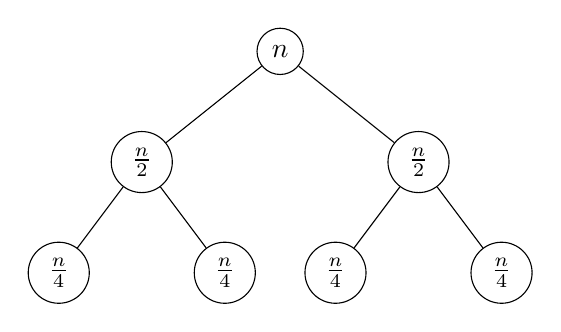
\begin{tikzpicture}[
  level distance=40 pt,
  every node/.style={circle,draw},
  level 1/.style={sibling distance=100 pt},
  level 2/.style={sibling distance=60 pt},
  level 3/.style={sibling distance=60 pt},
  level 4/.style={sibling distance=60 pt},
  level 5/.style={sibling distance=60 pt}
]
  \node {$n$}
    child {node {$\frac{n}{2}$}
    	child {node {$\frac{n}{4}$}}
    	child {node {$\frac{n}{4}$}}}
    child {node {$\frac{n}{2}$}
    	child {node {$\frac{n}{4}$}}
    	child {node {$\frac{n}{4}$}}};
\end{tikzpicture}
\end{center}

\subsubsection{Average-case Analysis of Quick Sort}
By our previous remark, we observe that the runtime is determined by the height $H$ of the tree that defines the depth of the recursive calls. This means that $T(n) \in O(n H(n))$. In the average case, $H(n) \in O(\log n)$, so the average-case runtime for this algorithm is $O(n \log n)$.\\
QuickSort is often the most efficient algorithm in practice.
%END%
\end{document}